\item[(e)]
\section{Magnitude and Phase Response}

\subsection*{Problem Statement}
Plot the magnitude and phase response of the filter.

\subsection*{Theoretical Background}
The frequency response of a digital filter can be analyzed by plotting its magnitude and phase responses. The magnitude response shows how the amplitude of each frequency component is modified by the filter, and the phase response shows the phase shift introduced by the filter at each frequency.

\subsection*{Implementation and Results}
The magnitude and phase response of the filter are computed and plotted using Python. The plots below illustrate the magnitude and phase response of the filter.

\begin{figure}[h]
    \centering
    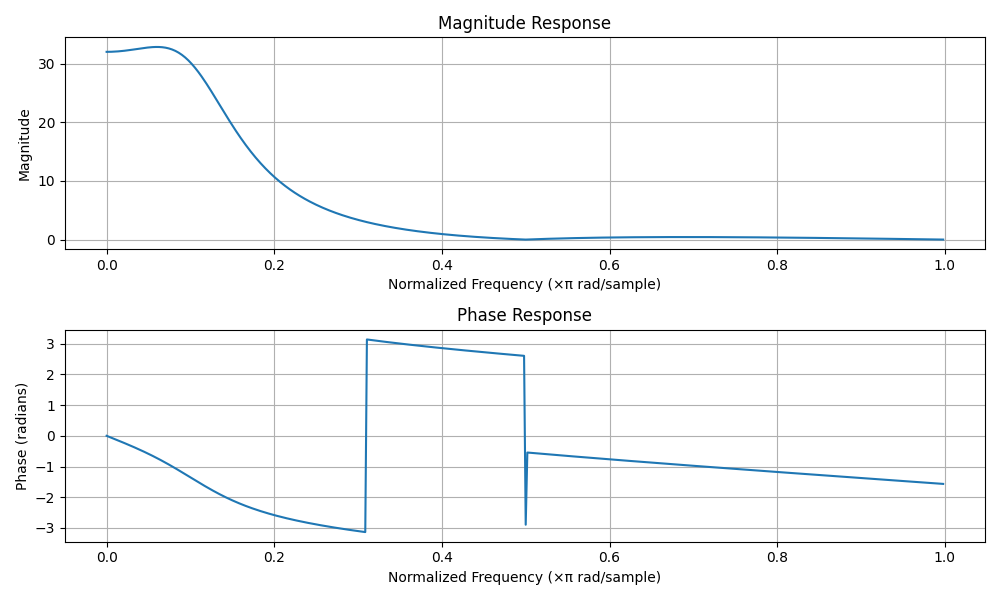
\includegraphics[width=0.8\textwidth]{fig/ex3_e_magnitude_phase_response.png}
    \caption{Magnitude and Phase Response of the Filter}
    \label{fig:ex3_e_magnitude_phase_response}
\end{figure}

\subsection*{Conclusion}
The magnitude and phase response plots provide insights into how the filter affects different frequency components of the input signal. The magnitude response shows the gain applied to each frequency, and the phase response shows the phase shift introduced by the filter.
